\documentclass[main.tex]{subfiles}
\begin{document}

\begin{figure}
\centering\fbox{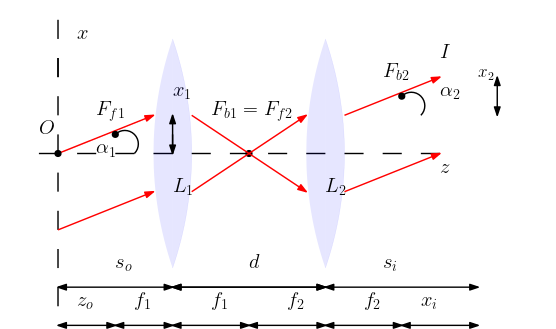
\includegraphics[height=2.0in]{figures/hw2/hw2_1.png}}
\caption{Parallel rays two lenses image formation variables spatial relationships}
\label{fig:2_1}
\end{figure}

\textbf{Exercise 1}\\

\textbf{Full Q} Parallel rays of elevation $x_1$ and propagation angle $\alpha_1$ are incident from the left on a two-lens system composed of two positive lenses $L1$ (focal length $f1>0$) and $L2$ (focal length $f2 >0)$ as shown in figure \ref{fig:2_1}.\\
1. What is the distance between the lenses ($d$) as a function of the focal lengths in order for the ray bundle outgoing from the second lens to be parallel? In other words, to obtain collimated beam; image at infinite? \textbf{Hint:} Use Image formation principle.\\
2. What is the optical power of this composite optical system and effective focal length (also referred to as \textbf{element focal length})? What is the value of the optical power for $d=f1+f2$? \textbf{Hint:} RTM?\\
3. What are the propagation angle $\alpha_2$ and width $a_2$ (defined as $x_2$ in the figure \ref{fig:2_1} and matrices) of this outgoing ray bundle? \\
4. What are the angular and lateral magnifications?\\
5.How is the image (virtual, real), what about the object? (Please point them out)?\\


\textbf{Intro} Parallel rays of elevation $x_1$ and propagation angle $\alpha_1$ are incident from the left on a two-lens system composed of two positive lenses $L1$ (focal length $f1>0$) and $L2$ (focal length $f2 >0)$ as shown in figure \ref{fig:2_1}.\\

\textbf{Q\&A 1} What is the distance between the lenses ($d$) as a function of the focal lengths in order for the ray bundle outgoing from the second lens to be parallel? In other words, to obtain collimated beam; image at infinite? \textbf{Hint:} Use Image formation principle.\\

When the collimated beam passes through bi-convex lens 1 it becomes a converging ray bundle with a focal length $f_1$. In order for the converging ray bundle from the perspective of the Lens 1 to act as an object point source diverging ray bundle which once passed through lens 2. The focal length $f_2$ needs to be at the same point as $f_1 \therefore d = f_1 + f_2$\\ 

%Due to the thin lens approximation, the lens thickness of $L_1$ and $L_2$ is negligible and $\therefore$ for elevation on either side of the lens $x_L = x_R = x$ . The system is surrounded by air with index $n_{air} = 1$. The ray transfer matrix for $L_1$ is


%\begin{equation}
%\begin{bmatrix}
%    \alpha_m \\
%    x_2
%\end{bmatrix}
%=
%\begin{bmatrix}
%    1   &   0 \\
%    d   &   1
%\end{bmatrix}
%\begin{bmatrix}
%    1   & -\frac{1}{f_1} \\
%    0   &   1
%\end{bmatrix}
%\begin{bmatrix}
%     \alpha_{1} \\
%    x_1
%\end{bmatrix}
%\end{equation}

%and the ray transfer matrix for $L_2$ is

%\begin{equation}
%\begin{bmatrix}
%    \alpha_2 \\
%    x_2
%\end{bmatrix}
%=
%\begin{bmatrix}
%    1   & -\frac{1}{f_2} \\
%    0   &   1
%\end{bmatrix}
%\begin{bmatrix}
%    \alpha_{m}  \\
%    x_2
%\end{bmatrix}
%\Rightarrow
%\begin{bmatrix}
%    1   & -\frac{1}{f_2} \\
%    0   &   1
%\end{bmatrix}^{-1}
%\begin{bmatrix}
%    \alpha_2 \\
%    x_2
%\end{bmatrix}
%=
%\begin{bmatrix}
%    \alpha_{m}  \\
%    x_2
%\end{bmatrix}
%\end{equation}

%substitution of matrix \ref{} into matrix \ref{} results in

%\begin{equation}
%\begin{bmatrix}
%    1   & -\frac{1}{f_2} \\
%    0   &   1
%\end{bmatrix}^{-1}
%\begin{bmatrix}
%    \alpha_2 \\
%    x_2
%\end{bmatrix}
%=
%\begin{bmatrix}
%    1   &   0 \\
%    d   &   1
%\end{bmatrix}
%\begin{bmatrix}
%    1   & -\frac{1}{f_1} \\
%    0   &   1
%\end{bmatrix}
%\begin{bmatrix}
%     \alpha_{1} \\
%    x_1
%\end{bmatrix}
%\end{equation}

%solve for reciprocal matrix, and multiplying the matrices 

%\begin{equation}
%\begin{bmatrix}
%    \alpha_2 + \frac{x_2}{f_2}\\
%    x_2
%\end{bmatrix}
%=
%\begin{bmatrix}
%    1   & -\frac{1}{f_1} \\
%    d   & 1 -\frac{d}{f_1}  
%\end{bmatrix}
%\begin{bmatrix}
%    \alpha_{1} \\
%    x_1
%\end{bmatrix}
%\end{equation}

%multiplying the right hand side matrices again

%\begin{equation}
%\begin{bmatrix}
%    \alpha_2 + \frac{x_2}{f_2}\\
%    x_2
%\end{bmatrix}
%=
%\begin{bmatrix}
%    \alpha_1 - \frac{x_1}{f_1} \\
%    d\alpha_1 + x_1 - \frac{x_1 d}{f_1}
%\end{bmatrix}
%\end{equation}

%solve for the column vectors on left and right side\\

%\begin{equation}
%\sqrt{(\alpha_2 + \frac{x_2}{f_2})^2 + (x_2)^2} = \sqrt{(\alpha_1 - \frac{x_1}{f_1})^2 + (d\alpha_1 + x_1 - \frac{x_1 d}{f_1})^2}
%\end{equation}

%square both sides of equation and solve for d

%\begin{equation}
%\begin{aligned}
%(\alpha_2 + \frac{x_2}{f_2})^2 + (x_2)^2 - (\alpha_1 - \frac{x_1}{f_1})^2 -x_1^2 & = d^2\alpha_1^2 + \frac{x_1^2 d^2}{f_1^2}\\ 
%                                                                              & + d \alpha_1 x_1 - \frac{x_1^2 d}{f_1} - \frac{x_1^2 d^2 \alpha_1}{f_1}
%\end{aligned}
%\end{equation}

%\begin{equation}
%\begin{aligned}
%(\alpha_2 + \frac{x_2}{f_2})^2 + (x_2)^2 - (\alpha_1 - \frac{x_1}{f_1})^2 -x_1^2 & = d^2(\alpha_1^2 + \frac{x_1^2}{f_1^2} - %\frac{x_1^2\alpha_1}{f_1})\\ 
%                                                                                 & + d(\alpha_1 x_1 - \frac{x_1^2}{f_1})
%\end{aligned}
%\end{equation}

%square both sides of equation and solve for d and expand \\

%Simplify with the knowledge that for the outgoing ray bundle from the second lens to be parallel $\alpha_1 = \alpha_2$ and $\therefore$ we %can relabel $\alpha_1 = \alpha_2 =\alpha$.\\

%\\ Trigonometrically we can state that $\tan(\alpha_m) = \frac{x_2}{d}$. For the outgoing ray bundle from the second lens to be parallel %$\alpha_1 = \alpha_2$.\\

%\fi

%\begin{equation}
%\begin{aligned}
%\alpha_2^2 + 2\frac{\alpha_2 x_2}{f_2} + \frac{x_2^2}{f_2^2} + x_2^2} = & \alpha_1^2 - 2\frac{\alpha_1 x_1}{f_1} + \frac{\alpha_1^2}{f_1^2} \\
% & + d^2\alpha_1^2 + x_1^2 + \frac{x_1^2 d^2}{f_1^2}\\ 
% & + d \alpha_1 x_1 - \frac{x_1^2 d}{f_1} - \frac{x_1^2 d^2 \alpha_1}{f_1}
%\end{aligned}
%\end{equation}


%solve for d

%\begin{equation}
%\begin{aligned%}
% \alpha_2^2 + 2\frac{\alpha_2 x_2}{f_2} + \frac{x_2^2}{f_2^2} + x_2^2}         & \\
% - \alpha_1^2 + 2\frac{\alpha_1 x_1}{f_1} - \frac{\alpha_1^2}{f_1^2} - x_1^2   & = d^2\alpha_1^2 + \frac{x_1^2 d^2}{f_1^2}\\ 
%                                                                               & + d \alpha_1 x_1 - \frac{x_1^2 d}{f_1} - \frac{x_1^2 d^2 \alpha_1}{f_1}
%\end{aligned}
%\end{equation}

%Simplify

%\begin{equation}
%\begin{aligned}
% \alpha_2^2 + 2\frac{\alpha_2 x_2}{f_2} + \frac{x_2^2}{f_2^2} + x_2^2}         & \\
% - \alpha_1^2 + 2\frac{\alpha_1 x_1}{f_1} - \frac{\alpha_1^2}{f_1^2} - x_1^2   & = d(d^2\alpha_1^2 + \frac{x_1^2 d^2}{f_1^2}\\ 
%                                                                               & + d \alpha_1 x_1 - \frac{x_1^2 d}{f_1} - \frac{x_1^2 d^2 \alpha_1}{f_1}
%\end{aligned}
%\end{equation}


\textbf{Q\&A 2} What is the optical power of this composite optical system and effective focal length (also referred to as \textbf{element focal length})? What is the value of the optical power for $d=f1+f2$? \textbf{Hint:} RTM?\\

When solving this problem we utilize Figure \ref{fig:2_1} to define ray transfer matrix Equation \ref{eq:2_1} where we are considering a telescope with infinite conjugates

\begin{equation}\label{eq:2_1}
\begin{bmatrix}
    \alpha_2 \\
    x_2
\end{bmatrix}
=
\begin{bmatrix}
    1   &   -\frac{1}{f_2} \\
    0   &   1
\end{bmatrix}
\begin{bmatrix}
    1   &   0 \\
    d   &   1
\end{bmatrix}
\begin{bmatrix}
    1   &   -\frac{1}{f_1} \\
    0   &   1
\end{bmatrix}
\begin{bmatrix}
    \alpha_{1} \\
    x_1
\end{bmatrix}
\end{equation}

Multiplying Matrices in Equation \ref{eq:2_1} results in Equation \ref{eq:2_2}.

\begin{equation}\label{eq:2_2}
\begin{bmatrix}
    \alpha_2 \\
    x_2
\end{bmatrix}
=
\begin{bmatrix}
    1 - \frac{d}{f_2}   &  \frac{d}{f_1 f_2} - \frac{1}{f_1} - \frac{1}{f_2} \\
    d                   &   1 - \frac{d}{f_1}
\end{bmatrix}
\begin{bmatrix}
    \alpha_{1} \\
    x_1
\end{bmatrix}
\end{equation}

Where the optical power $P$ is defined in Equation \ref{eq:2_3}

\begin{equation}\label{eq:2_3}
P = \frac{d}{f_1 f_2} - \frac{1}{f_1} - \frac{1}{f_2} = - \frac{(f_1+f_2)-d}{f_1 f_2}
\end{equation}

and the effective focal length $EFL$ is defined in Equation \ref{eq:2_4}.

\begin{equation}\label{eq:2_4}
EFL = -\frac{1}{P} = \frac{f_1 f_2}{(f_1+f_2)-d}
\end{equation}

For $d = f_1 + f_2$ the optical power $P = - \frac{(f_1+f_2)-d}{f_1 f_2} = - \frac{(d)-d}{f_1 f_2} = 0$ and the focal length is $\infty$ resulting in a collimated beam and expressed in ray transfer matrix Equation \ref{eq:2_5}.

\begin{equation}\label{eq:2_5}
\begin{bmatrix}
    \alpha_2 \\
    x_2
\end{bmatrix}
=
\begin{bmatrix}
    1 - \frac{d}{f_2}   &  0 \\
    d                   &  1 - \frac{d}{f_1}
\end{bmatrix}
\begin{bmatrix}
    \alpha_{1} \\
    x_1
\end{bmatrix}
\end{equation}

%Optical power is equal to the reciprocal of the focal length of the device $P=\frac{1}{f}$. The element focal length for a two lens system is defined as $EFL = \frac{f_1 \times f_2}{f_1 + f_2 - d}$ $\therefore$ the optical power of a two lens system is defined as $P=\frac{f_1 + f_2 -d}{f_1 \times f_2}$ and $\therefore$ the optical power for $d=f_1 + f_2$ is shown to be $P=\frac{f_1 + f_2 - (f_1 + f_2)}{f_1 \times f_2} = 0$\\

\textbf{Q\&A 3} What are the propagation angle $\alpha_2$ and width $a_2$ (defined as $x_2$ in the figure \ref{fig:2_1} and matrices) of this outgoing ray bundle given that $d=f_1 + f_2?\\

Using Equation \ref{eq:2_5} we calculate $\alpha_2$ in Equation \ref{eq:2_6}

\begin{equation}\label{eq:2_6}
\alpha_2 = (1-\frac{d}{f_2})\alpha_1 = (1-\frac{f_1}{f_2} - \frac{f_2}{f_2})\alpha_1 = \frac{-f_1}{f_2}\alpha_1 
\end{equation}

and we calculate $x_2$ in Equation \ref{eq:2_7} where for $\alpha_1 = 0$, $x_2 = -\frac{f_2}{f_1}x_1$.

\begin{equation}\label{eq:2_7}
x_2 = d \alpha_1 + (1-\frac{d}{f_1})x_1 = (f_1 +  f_2)\alpha_1 + \frac{f_1 - d}{f_1}x_1
\end{equation}

%$\alpha_2$ and width(z in Joseph Crandall's coordinate system) $z_2$ are spatially indicated in figure \ref{fig:2_1}.\\
%The ray transfer matrix for the $L_1$, $L_2$ telescope system is

%\begin{equation}
%\begin{bmatrix}
%    \alpha_2 \\
%    x_2
%\end{bmatrix}
%=
%\begin{bmatrix}
%    1   & -\frac{1}{f_2} \\
%    0   &   1
%\end{bmatrix}
%begin{bmatrix}
%    1   &   0 \\
%    d   &   1
%\end{bmatrix}
%\begin{bmatrix}
%    1   & -\frac{1}{f_1} \\
%    0   &   1
%\end{bmatrix}
%\begin{bmatrix}
%    \alpha_{1}  \\
%    x_1
%\end{bmatrix}
%\end{equation}


\textbf{Q\&A 4} What are the angular and lateral magnifications?\\

The angular magnification is defined as $M_A = \frac{-s_o}{s_1} = \frac{\alpha_2}{\alpha_1} = -\frac{f_1}{f_2}$ and the lateral magnification (sometimes called linear or transverse) is defined as $M_T = \frac{-s_i}{s_o} = \frac{x_2}{x_1} = \frac{-f_2}{f_1} = \frac{1}{M_A}$. $s_o$ and $s_i$ are indicated spatially in figure \ref{fig:2_1}\\

\textbf{Q\&A 5} How is the image (virtual, real), what about the object? (Please point them out)\\

At great object $O$ distances the incident rays are effectively parallel and the object is real. The image $I$ is spatially indicated in figure \ref{fig:2_1} and the final image is virtual, enlarged, and inverted. 

In the case of infinite conjugates telescope the image is at infinite and the object is real at infinite distance. The intermediate image is at finite distance lens $1$ from $L_1$ and $f_2$ from lens $2$.



\newpage

\begin{figure}
\centering\fbox{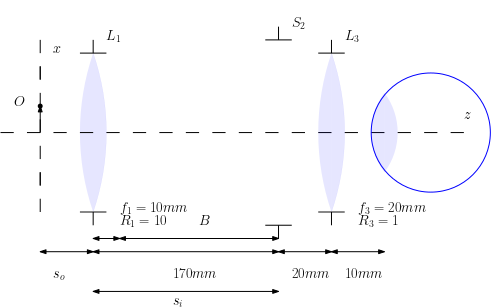
\includegraphics[height=2.0in]{figures/hw2/hw2_2.png}}
\caption{Spatial Relationships between lens, aperture, lens, and eye}
\label{fig:2_2}
\end{figure}

\textbf{Exercise 2}\\
The optical instrument shown below consists of 2 lenses $L_1$, $L_3$ and an aperture stop $S_2$ and the observer's eye is located to the right of $L_3$. Symbols $\{f_1 , R_1\}$ , $\{f_3 , R_3\}$ represent the focal lengths and radii of $L_1$, $L_3$, respectively, and $R_2$ is the radius of $S_2$ \ref{fig:2_2}.\\

\textbf{Q\&A} Determine the object distance so that a human observer's unaccommodating eye (no strain for focusing) can focus the image on the observer's retina. \textbf{Hint:} this means outgoing parallel ray bundle from $L_3$, which means that lens $1 ...$\\

... must have incident object $O$ at finite distance $s_0$. The Huygens eyepiece ($L_3$) also know as the "ocular" is a magnifier meant to look at the intermediate image formed by the preceding optical instrument. The eye looks into the eyepiece, and the eyepiece "looks" into the optical system, in this case a compound microscope with an aperture (field stop) $S_2$ and an Objective lens $L_1$.\\

The objective lens forms a real, inverted magnified image of the object. The image resides in space on the plane of the field stop of the eyepiece and has to be small enough to fit inside the barrel of the device, denoted by $B=160mm$. The lateral magnification of the objective lens requires that $\frac{h_i}{h_0} = \frac{-f}{x_0} = -\frac{x_i}{f} \because$ Newton's Formula states that $x_o x_i = f^2$. Lateral magnification of the Objective lens also defines that $\frac{h_i}{h_0} = -\frac{s_i}{s_o}$ which when combined form the Image Condition

\begin{equation}
\frac{s_i}{s_o} = \frac{f}{x_o} = \frac{f}{s_o - x_o} \Rightarrow \frac{1}{s_o} \frac{1}{s_i} = \frac{1}{f} \Rightarrow s_o = \frac{10mm}{170mm} = \SI{58.824}{\mu \meter} 
\end{equation}


If the object is placed \SI{58.824}{\mu \meter} away from the objective lens, the image formed on the aperture will contain Rays diverging from each point of this image and will emerge from the eye-lens (which in this simple case is the eyepiece itself).\\ 


Ideally this should produce a virtual image at $\infty$ such that the Magnification is defined as $MP=d_0P$ so that the final image is viewed with a relaxed (unaccommodated) eye, and so as to center the exit pupil (eye point) where the observer's eye is placed at $10mm$ (eye relief) from the instrument.\\

\fi

\textbf{Q\&A} What is the instrument use and what is the magnifying power? \textbf{Hint:} small object viewed by an eye.\\

The instrument is a rudimentary compound microscope and the Magnification power of the entire system is the product of the transverse linear magnification of the objective $M_T$, and the angular magnification of the eyepiece, $M_A$, forming the equality $M = M_{To} M_{Ae} = \frac{-x_i}{f_o} \frac{x_o}{f_e} = \frac{-B}{f_1} \frac{?}{f_3} = \frac{-160}{10} \frac{250}{20} = 200$. The objective magnifies the object and brings it up in the form of a real image, where it can be examined as if through a magnifying glass.

%\textbf{What is the standard near point}. 

\end{document}